% 1D Dirichlet sine decay -- case.py (energy-coupled, EOS temperature).
% The sine profile is imposed through the DENSITY at uniform pressure,
%   rho(x) = rho0 Twall / (Twall + A sin(pi x/L)),   p = p0 = const.
% T is then recovered from the stiffened-gas EOS; weak compressible acoustics
% make u != 0 and set a small physics-driven error floor.
%
% Compile:  pdflatex setup_1d.tex
\documentclass[border=12pt]{standalone}
\usepackage{amsmath}
\usepackage{tikz}
\usepackage{pgfplots}
\pgfplotsset{compat=1.18}
\usetikzlibrary{arrows.meta, calc}

\definecolor{coldc}{RGB}{46,86,149}
\definecolor{hotc}{RGB}{171,57,52}
\definecolor{inkc}{RGB}{30,30,30}
\definecolor{rhoc}{RGB}{109,72,140}

\begin{document}
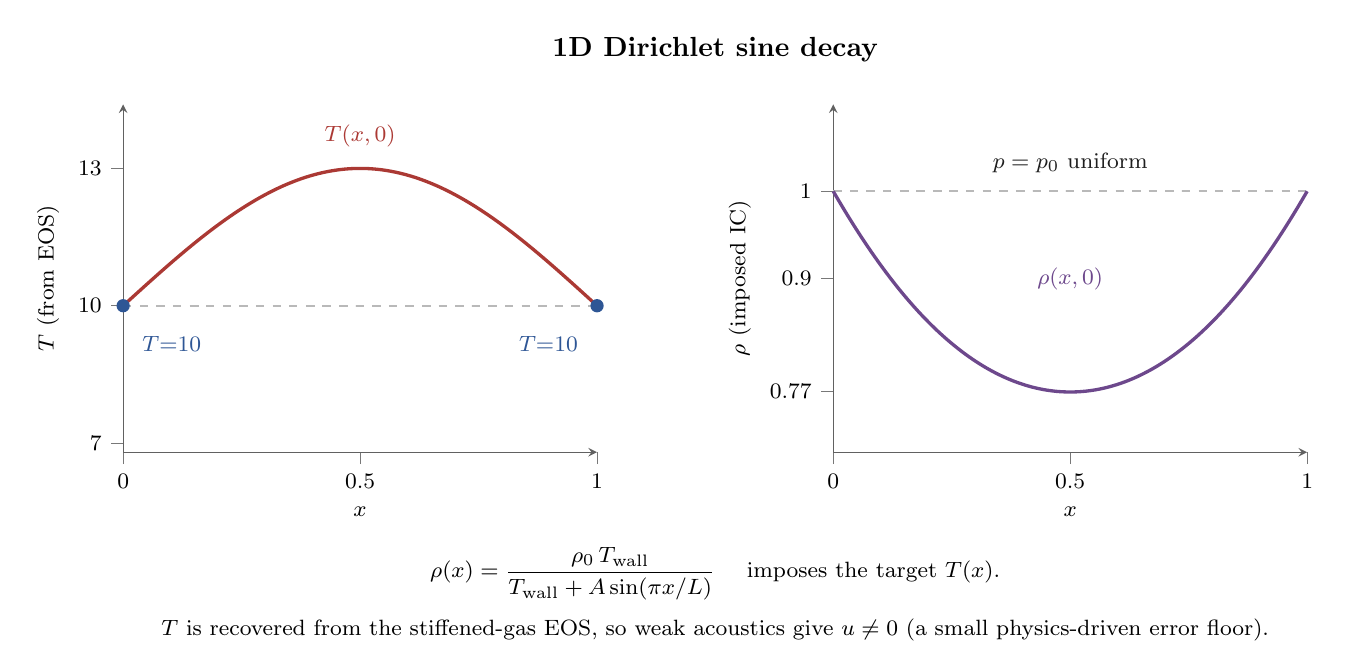
\begin{tikzpicture}[>=Stealth, font=\footnotesize]
\pgfplotsset{
  panel/.style={
    width=7.6cm, height=6.0cm, axis lines=left, samples=160,
    xmin=0, xmax=1, xtick={0,0.5,1}, enlargelimits=false, clip=false,
    xlabel={$x$}, every axis x label/.style={at={(ticklabel cs:0.5)}, anchor=north},
    tick align=outside, tick style={inkc!60}, axis line style={inkc!70},
  },
}

% LEFT panel: recovered temperature T(x)
\begin{axis}[panel, name=tax,
  ylabel={$T$ (from EOS)}, ymin=6.8, ymax=14.4, ytick={7,10,13},
]
  \addplot[gray!55, dashed, thick, domain=0:1] {10};
  \addplot[hotc, very thick, domain=0:1] {10 + 3*sin(deg(pi*x))};
  \node[hotc, anchor=south] at (axis cs:0.5,13.25) {$T(x,0)$};
  \fill[coldc] (axis cs:0,10) circle (2.4pt);
  \fill[coldc] (axis cs:1,10) circle (2.4pt);
  \node[coldc, anchor=north west] at (axis cs:0.02,9.55) {$T{=}10$};
  \node[coldc, anchor=north east] at (axis cs:0.98,9.55) {$T{=}10$};
\end{axis}

% RIGHT panel: imposed density rho(x) (inverse of T at uniform pressure)
\begin{axis}[panel, name=rax, at={(tax.east)}, anchor=west, xshift=3.0cm,
  ylabel={$\rho$ (imposed IC)}, ymin=0.70, ymax=1.10, ytick={0.77,0.9,1.0},
]
  \addplot[gray!55, dashed, thick, domain=0:1] {1.0};
  \addplot[rhoc, very thick, domain=0:1] {10/(10 + 3*sin(deg(pi*x)))};
  \node[rhoc, anchor=south] at (axis cs:0.5,0.875) {$\rho(x,0)$};
  \node[inkc, anchor=south] at (axis cs:0.5,1.01) {$p=p_0$ uniform};
\end{axis}

% Centered title above both panels
\node[font=\bfseries] at ($(tax.north)!0.5!(rax.north) + (0,0.7cm)$)
  {1D Dirichlet sine decay};

% Centered caption below both panels
\node[anchor=north, align=center, inner sep=0pt]
  at ($(tax.south)!0.5!(rax.south) - (0,1.2cm)$)
  {$\displaystyle \rho(x)=\frac{\rho_0\,T_{\text{wall}}}{T_{\text{wall}}+A\sin(\pi x/L)}$
   \quad imposes the target $T(x)$. \\[6pt]
   $T$ is recovered from the stiffened-gas EOS, so weak acoustics give $u\neq 0$
   (a small physics-driven error floor).};
\end{tikzpicture}
\end{document}
